\documentclass[12pt, a4paper]{article}

\usepackage{setspace, graphicx, caption, color, float}
\usepackage{amsmath}
\usepackage{amsfonts}
\usepackage{amssymb}
\usepackage{amsthm}
\usepackage{amstext} %to enter text in mathematical formulae
\usepackage[retainorgcmds]{IEEEtrantools}
\usepackage{natbib}
\usepackage{hyperref} % for linking refferences to supps
\usepackage{lineno} % for line numbers, need it after amsmath

%page set up
\usepackage[left=2.5cm,top=2.5cm,right=2.5cm, bottom=2.5cm,nohead]{geometry}
\doublespacing
%paragraph formatting
\setlength{\parskip}{12pt}
\setlength{\parindent}{0cm}

\linenumbers

\begin{document}
Title: Optimal control in the face of evolving resistance is an economic problem not a biological one.

Shaun R. Coutts, Helen Hicks, Alexa Varah, Kwadjo Ahodo, Rob Frekleton, Dylan Z. Childs 

\newpage

\section*{Abstract}
Evolved resistance to xenobiotics (e.g. antibiotics, herbicides, pesticides, fungicides) is a global threat to public health and food security. In agricultural systems non-chemical control methods can be combined with xenobiotics (Integrated Pest Management; IPM) to prolong the useful life of compounds and manage pest populations after resistance has evolved. We find IPM strategies with the highest economic returns for an arable cropping system, and perform a global sensitivity analysis to find the factors that shape those strategies. The key uncertainties are economic in nature, and farmers have an incentive to be responsive to changes in the shape of the yield loss function. Doing so effectively will require estimating, at a minimum, what yields would be in the absence of the pest, maximum weed density and how yields change with increasing pest density, with enough detail to say how much control (if any) is justified.            

\section*{Significance}
Integrated pest management (IPM) applies chemical and non-chemical control methods to pest populations to manage evolved resistance. Surprisingly, despite the widespread adoption of IPM, we have a poor understanding of how to select between alternative IPM strategies. Here we consider a typical problem, a farming system in which high levels of herbicide resistance evolves repeatedly. The best IPM strategies were dependent on crop yields, yield loss caused by the weed and the maximum possible loss, land tenure, and levels of herbicide resistance. With the exception of herbicide resistance, all these factors are economic in nature, thus knowing which IPM strategy to apply where is an economic problem rather than biological one.

\newpage

\section*{Introduction}
Controlling populations in the face evolving resistance to xenobiotics (i.e. antibiotics, herbicides, pesticides, fungicides) is one of the biggest challenges facing public health \citep{Laxm2016, Willy2017}, and food security \citep{Denh1992, Palu2001, Hick2018}. Evolved resistance also costs billions of dollars globally \citep{Livi2016, Ches2018, Hick2018}. In agricultural systems evolved resistance can be mitigated with integrated pest management (IPM), where chemical control is used in combination with non-chemical techniques such as crop rotation, cultivation and spot control (e.g. hand-weeding). IPM can be used both pro-actively to delay the evolution of resistance, and reactively to control pest populations as chemical control becomes less effective \citep{Denh1992, Hick2018}. However, while the concept of IPM is well established \citep{Bott1979}, finding cost effective IPM strategies is extremely challenging \citep{Dana2014, Chal2015}. Management tools need to be used in the correct combination and sequence to be effective. This results in a very large number of potential IPM strategies (i.e. different combinations and sequences), even when considering only a handful of management tools and short time horizons \citep{Chal2015}. 

As a result of this difficulty, there have been no attempts to rigorously search for cost effective IPM strategies in the face of rapidly evolving resistance to one of the primary management options. This is an important gap in our understanding for agricultural systems; where resistance to xenobiotics has evolved numerous times \citep{Denh1992, Palu2001} and multiple non-chemical control options can be used in combination to deliver cost effective control \citep{Chal2015}.      

Further, little is known about how robust good IPM strategies are to changes in factors such as crop yield and pest population dynamics \citep{EpanN2010}. Thus, even when effective IPM strategies are found, we do not know how generally we should expect them to apply. Ideally we would find IPM strategies that are robust to changes in factors that change between fields, like crop yields \citep{Swin1994, Hick2018}, so that standard IPM strategies can be applied across entire farms or regions. If we cannot find robust IPM strategies then farmers face the prospect of having to find workable IPM strategies for each field. This would pose a serious barrier to IPM adoption, as IPM strategies are already seen as complex and difficult to implement \citep{Llew2006}. An alternative is to find a small set of easily measurable factors that shape IPM strategies in predictable ways. So that even if cost-effective IPM strategies do change from field to field, it is at least straight forward to know which strategy to apply where.     

We used \textit{Alopecurus myosuroides} as a test case. \textit{A. myosuroides} is Europe's most economically costly weed \citep{Moss2007} and one of the worlds most serious herbicide resistant grass weeds \citep{Heap2014}. Herbicide-resistant \textit{A. myosuroides} costs up to \pounds 320$\cdot$ha$^{-1}$ in yield loss and extra herbicide use \citep{Hick2018}, and imposes a total cost of \pounds 0.5bn across England (Varah et al, in press). We built a population model for \textit{A. myosuroides} where target site resistance to two herbicides is already present, although possibly at very low frequencies. While most current strategies to mitigate resistance focus on delaying resistance \citep{REX2013}, in many agricultural weeds, including \textit{A. myosuroides}, herbicide resistance is already widespread \citep{Hick2018}.            

We framed IPM as a combinatorial optimisation problem and used a genetic algorithm (Appendix 1) to find economically incentivised (measured by gross margin) IPM strategies \citep{Tayl2004GA, Carr2010} in the face of evolution. We carried out the first global sensitivity analysis of dynamic IPM strategies (Appendix 2), testing how robust those IPM strategies were across 15,000 parameter combinations incorporate a wide range of economic, biological and psychological factors. We find that cost effective IPM strategies can change dramatically in response to changes in potential yield losses, but a small number of parameters predicted how those cost effective IPM strategies changed. 

\section*{Results and Discussion}
To find which parameters were crucial in shaping IPM with high gross margin we used multi-variate boosted regression trees \citep{Mill2016} as a meta-model \citep{Cout2013}(Appendix 2). We interrogated this meta-model to find important parameters accounting for high-level interactions and non-linear responses \citep{Frie2001, Mill2016}.

Across a wide range of parameter combinations the key uncertainties related to the economic impact of the weed, despite much research on IPM focusing on biological factors \citep{Colb2006}. In particular parameters defining the yield loss function (Fig. \ref{fig:rel_inf}) had the most influence on shaping incentivized IPM strategies. The yield loss function describes the relationship between weed density and crop yield. Yield when the weed was absent ($Y_0$) and the effect of weed density on yield ($Y_D$) were two of the most important parameters (Fig. \ref{fig:rel_inf}). Another set of parameters that control how large the seed bank can become ($f_m$, $f_d$ and $\phi_b$; Fig. \ref{fig:rel_inf}) were also important. The potential size of the seed bank sets the maximum possible loss if the weed population is uncontrolled. Although yield loss functions have been estimated for major weeds \citep{Cous1985, Doyl1986, Swin1994}, there is evidence that yield functions vary substantially between fields \citep{Swin1994, Hick2018}, and little attention has been paid to this variation and understanding its causes.
 \begin{figure}
	\centering
	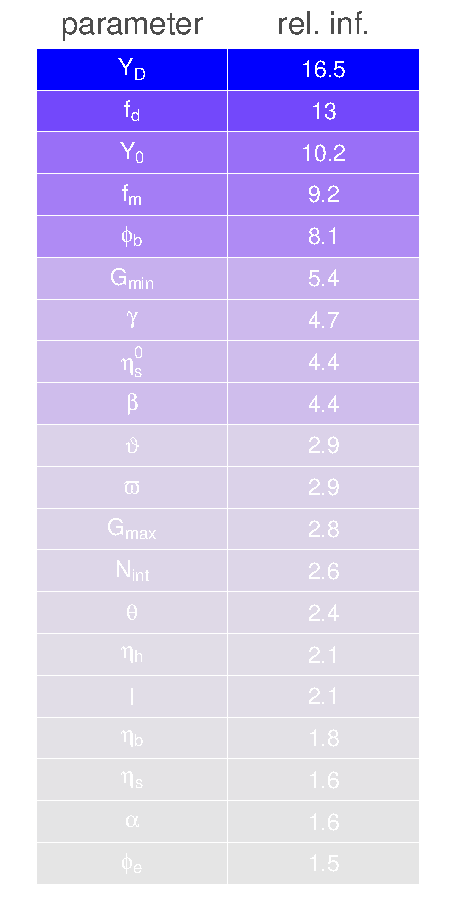
\includegraphics[height=80mm]{MS_figs/rel_inf_mean.pdf}
	\caption{Relative influence of each parameter on IPM strategy (Appendix 2). Relative influence is the reduction in mean squared error attributable to each parameter. Because only values are only meaningful relative to each other the relative influence index is re-scaled to sum to 100 across all parameters \citep{Frie2001, Mill2016}. Higher values indicate parameters with more influence on the structure of incentivized IPM strategies.}
	\label{fig:rel_inf} 
\end{figure}

While the shape of the yield loss function is important because it determines how much control is justified, knowing which type of IPM strategy to employ may only require an estimate of yield in the absence of the weed ($Y_0$), and one or two thresholds values of weed density where a new IPM strategy becomes advantageous. When the yield of winter wheat with no \textit{A. myosuroides} ($Y_0$) was low, management intensity was lower and relied on crop rotation and tactical use of herbicide (Fig. \ref{fig:Y0_YD}, '$Y_0$ low'). The strategy changed little when the effect of weed density on yield ($Y_D$) increased. Although, more herbicide was used when the value of $Y_D$ increased from a very low value to a slightly higher value (1\% to 12\% losses at high densities of \textit{A. myosuroides}; Fig. \ref{fig:Y0_YD}g,e). When $Y_0$ was high, $Y_D$ showed two thresholds where IPM strategy changed. When $Y_D$ was very low relative to the maximum \textit{A. myosuroides} population possible, the best strategy was to do noting and live with high populations of \textit{A. myosuroides} (Fig. \ref{fig:Y0_YD}h). Since yield losses were never high enough to justify expenditure on control. Increasing $Y_D$ slightly meant some herbicide use and cultivation to rotate the seed bank became advantageous (Fig. \ref{fig:Y0_YD}f). Once $Y_D$ increased enough to justify intensive control, further increases did not change the IPM strategy (Fig. \ref{fig:Y0_YD}b,d). 
\begin{figure}
	\centering
	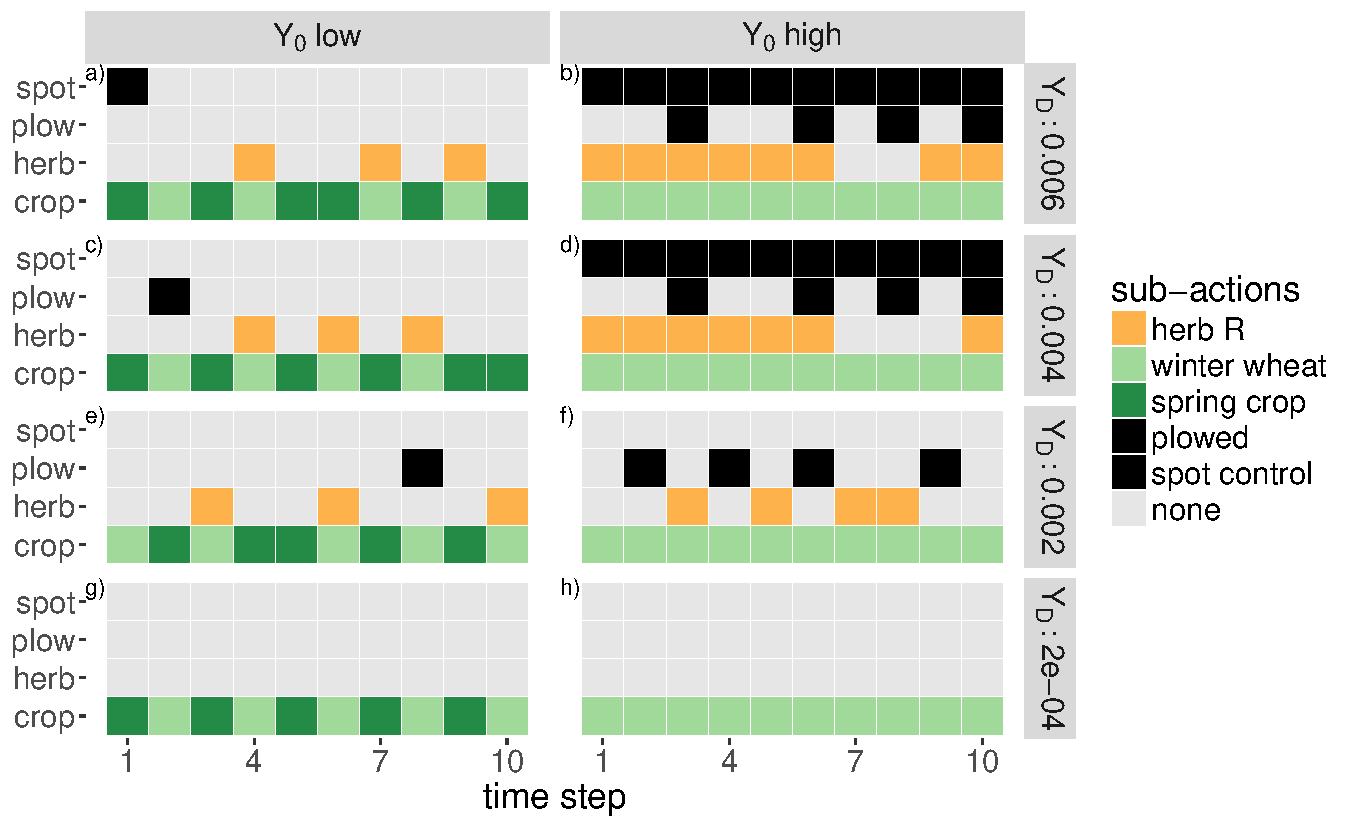
\includegraphics[width=1\linewidth]{MS_figs/MS_act_seq_YD_Y0.pdf}
	\caption{IPM strategies under high (\pounds 1668$\cdot$ha$^{-1}$) and low (\pounds 986$\cdot$ha$^{-1}$) values of $Y_0$ (yield of winter wheat with no \textit{A. myosuroides}), under increasing values (rows) of $Y_D$ (in \pounds$\cdot$plant$^{-1}\cdot$ha$^{-1}$). At the lower limit of $Y_D$ very high \textit{A. myosuroides} densities result in a 1\% yield loss under the high $Y_0$ scenario, and the upper limit implies a yield loss of 35\%. There is initially one effective herbicide ($R_\text{int} = 0.0001$, $Q_\text{int} = 0.9$). We used partial dependence plots to explore how different parameter combinations change IPM strategy. Partial dependence plots show the marginal effect of a parameter of interest on IPM strategy \citep{Frie2001, Mill2016}. Once relevant parameter ranges were found we re-ran the genetic algorithm for those parameter combinations to generate actual IPM strategies rather than the marginal effects.}
	\label{fig:Y0_YD} 
\end{figure}

Intensive management can be costly, and so require returns over several years to justify. As a result valuing returns further into the future (in our model controlled by the discount rate $\gamma$) encourages more intensive management \citep{EpanN2010}. Intensive management to reduce the seed bank was only selected by the genetic algorithm when future returns were given more value (higher values of $\gamma$, Fig. \ref{fig:dis_rate}). In agricultural systems land tenure has a crucial effect on how investments in weed control are valued. Those who own fields can benefit from long-term investments like weed control campaigns and soil conservation, whereas those who rent fields do not \citep{Wies1996, Fras2004}. The amount of rented farm land can be considerable. In 2014 54\% of crop land in the USA was rented \citep{Bige2016}, and 35\% of all agricultural land in England and Wales is rented \citep{CAAV2017}. This has important implications for the level of control managers are incentivised to provide, and thus the spread and the evolution of resistance \citep{Mare2012}.       
\begin{figure*}
	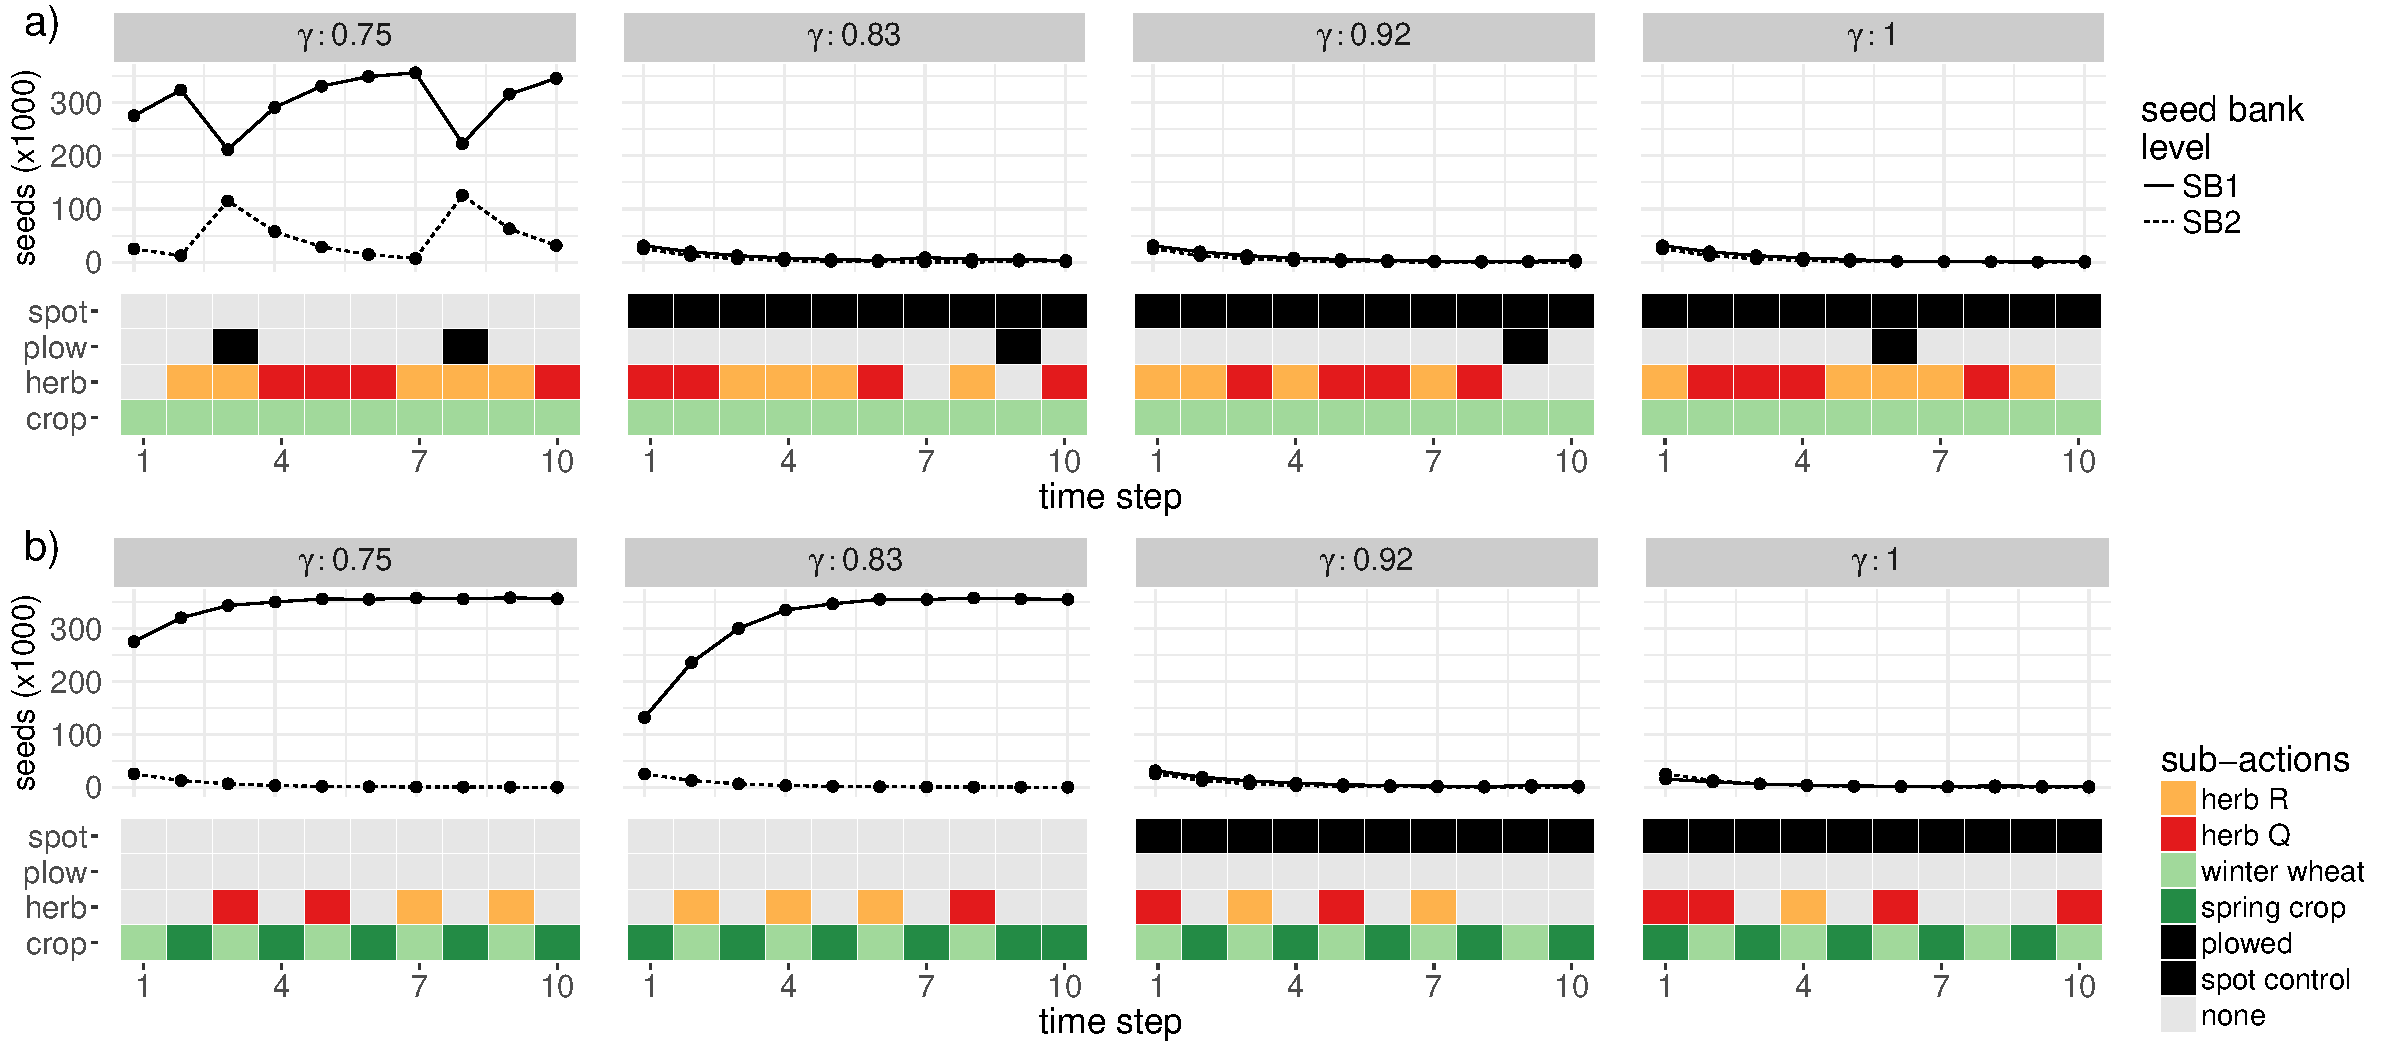
\includegraphics[width=178mm]{MS_figs/dis_rate_SB_strat.pdf}
	\caption{The effect of discount rate ($\gamma$) on the seed bank and IPM strategy (tile plots) when yields from winter wheat are high (a; \pounds 1668$\cdot$ha$^{-1}$) and low (b; \pounds 986$\cdot$ha$^{-1}$). When $\gamma = 0.75$ rewards 5 years in the future are valued at 23\% of current returns and when $\gamma = 1$ present and future rewards are valued equally. In both cases the slope of the yield function ($Y_D$) is high (\pounds 0.006$\cdot$plant$^{-1}\cdot$ha$^{-1}$). Initial resistance was low for both herbicides. Although we only show the first 10 years of IPM strategy, the discounted returns over 25 years are considered by the genetic algorithm.}
	\label{fig:dis_rate} 
\end{figure*}

Resistance increased quickly with herbicide use. Even starting at low frequencies, high levels of resistance evolved after just seven herbicide applications (Fig. \ref{fig:int_res}b). The best IPM strategies found were responsive to increasing resistance, drastically reducing herbicide use as higher levels of resistance evolved (Fig. \ref{fig:int_res}b--d). In contrast, multiple herbicide applications per year are the norm in this cropping system, despite high levels of resistance \citep{Hick2018}. This disparity could arise from a number of contributing factors. Some managers may believe that even a little control (mortality of a few susceptible individuals) is better than no control and inaction is seen as the worst approach to weed management \citep{Wils2008}. In addition, IPM strategies are often seen as complex in comparison to routine application of chemicals, and having a steep learning curve \citep{Llew2006}. Resistance tends to be partial and build up slowly \citep{Moss2009, Hull2014}, so farmers may be victims of a shifting baseline, lowering their expectations of efficacy of weed control. There may be a belief that new herbicides will become available, despite no new modes of action being marketed for over 20 years \citep{Duke2012}. Thus, current strategies are viewed as a bridging strategy until a new product is found \citep{Hurl2016}. Finally, Our population model was deterministic, so IPM strategies could not be risk averse to variability in \textit{A. myosuroides} populations and economics factors like crop prices. Uncertainty in when herbicide resistance will emerge and the efficacy of non-chemical control can be a major impediment to adopting IPM \citep{Hurl2016}.     

In our system herbicide resistance incurred a high cost, and even the best IPM strategies found saw their gross margin (reward) reduced by upto a quarter once high levels of resistance had evolved (Fig. \ref{fig:int_res}c,d). These losses had different sources depending on the initial resistance. When initial resistance was low the weed population could be initially reduced with herbicide, but required more expensive non-chemical control to keep the weed population low so that spot control remained feasible (Fig. \ref{fig:int_res}c). When resistance was high there were few effective control options and high weed populations reduced the yield (Fig. \ref{fig:int_res}c). It should be noted this result depends on the yield loss function. If high densities of the weed do not cause large yield loses then high levels of resistance are less of a concern, and high expenditure on non-chemical control is not justified.           

Much work on managing resistance focuses on delaying its establishment in the population, and in such cases both stacking and cycling compounds can be effective \citep{REX2013}. In contrast we modelled reactive management, where resistance is already established in the population \citep{Hick2018}. Over a wide range of parameters, when both herbicides were effective the preference was to cycle between them (e.g. Fig. \ref{fig:dis_rate} and \ref{fig:int_res}a). Cycling was favoured over stacking because the application of each herbicide was spread out, prolonging their life.

We present the best case that can be hoped for in reactive management, as we assume that herbicide resistance was conferred by target site mutations. However, there is growing evidence that non-target site resistance, which confers cross resistance, is widespread \citep{Hick2018}. If generalized, non-target site resistance mechanisms are present, the total amount of herbicide exposure predicts resistance level \citep{Hick2018}, and cycling will not help.
\begin{figure*}[!ht]
	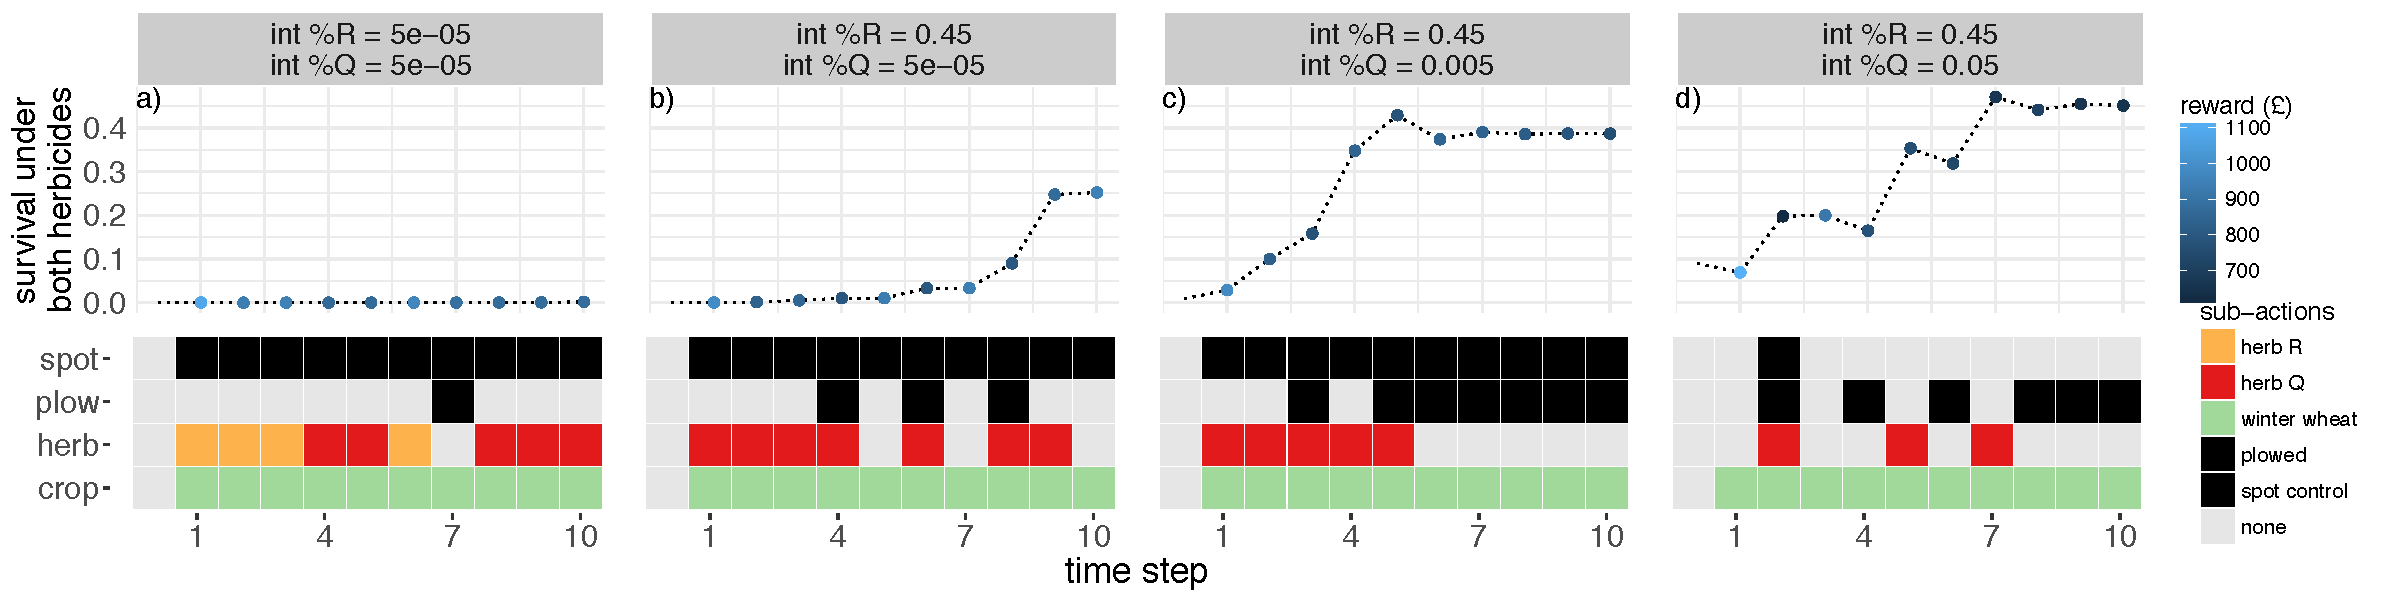
\includegraphics[width=178mm]{MS_figs/int_res_strat_resist.pdf}
	\caption{The effect of initial resistance on the selected IPM strategy (tile plots) and the evolution of herbicide resistance (\% survival to under both herbicides). Lighter coloured points indicate higher reward (gross margin) obtained in that time step. In this case $Y_0 = 1668$ (high winter wheat yield) and $Y_D = 0.0062$ (high yield penalty).}
	\label{fig:int_res} 
\end{figure*}

We assume that herbicide is the only action that drives the evolution of resistance. Any effective management tool will impose selection pressure, and so drive resistance to that tool. In reality, the spring cropping and spot control sub-actions make heavy use of glyphosate to control \textit{A. myosuroides}. Glyphosate resistance has evolved on many separate occasions in response to prolonged, heavy use \citep{Samm2014}. As glyphosate becomes a more important part of weed management \citep{Hick2018} resistance is likely. 

\section*{Conclusion}
Combating xenobiotic resistance is ultimately a problem of behaviour change, and thus how individuals are incentivized to act \citep{Hurl2016}. Our results show that farmers have an economic incentive to be responsive to changes in the shape of the yield loss function. Doing so will require estimating, at a minimum, what yields would be in the absence of the pest, and how yields change with increasing pest density, with enough detail to say how much control (if any) is justified. The most salient piece of data on the weed population is its maximum density, as this sets the maximum possible yield loss.      

[ALEXA: would be nice to conclude with a nice summary statement on what a failure to be responsive will cost farmers, the economy as whole and the environment, are at least as much as we can say at this point. Also be a good place to flag your up coming work for any things that are still unresolved. If it is all unresolved that is an important message as well I think.] 

\subsection*{Data Archival}

PNAS must be able to archive the data essential to a published article. Where such archiving is not possible, deposition of data in public databases, such as GenBank, ArrayExpress, Protein Data Bank, Unidata, and others outlined in the Information for Authors, is acceptable.

\subsection*{Supporting Information (SI)}
\subsubsection*{Appendices}
Appendix 1: Genetic Algorithm\\
Appendix 2: Finding Which Initial Conditions and Model Parameters Lead to Which IPM Strategies\\
Appendix 3: Action Space\\
Appendix 4: Population Model\\
Appendix 5: Reward Function\\

\section*{Methods}
We frame IPM as a combinatorial optimisation problem where the goal is to find a good combination of management tools, used in sequence. We use a genetic algorithm to solve this combinatorial problem \citep{Tayl2004GA, Carr2010}. Genetic algorithms cannot be checked to have found the globally optimal solution, as this would require already knowing the solution; however, genetic algorithms are efficient at selecting out comparatively poor solutions, so that over successive iterations the regions of the solution space being explored gets progressively better, resulting in a set of good (often near optimal) solutions.

Our goal is to find good IPM strategies in the face of rapidly evolving resistance, and how those strategies change in response to biological and management parameters. This problem has fours parts: i) a reward function that measures how good a given IPM strategy is based on how much that strategy costs and its effectiveness, we use net present economic value; ii) a population model that translates a given IPM strategy into a population, and thus a reward; iii) an algorithm that finds IPM strategies with higher rewards, the genetic algorithm (Appendix 1); iv) finally we need to relate changes in the best IPM strategy found to changes in initial conditions and model parameters. For this we use a meta-modelling global sensitivity analysis \citep{Cout2014} based on multi-variate boosted regression trees \citep{Mill2016}. 

\subsection*{Population model}
The population model links management actions to the response of the \textit{A. myosuroides} population, and thus wheat yields. Each action $a_j$ is a tuple of four sub-actions $a_j = \langle a_h, a_b, a_k, a_s \rangle$. See Appendix 3 for a description of the sub-actions and all eligible combinations of these sub-actions (i.e. the full actions space, $\mathbf{A}$). 

The processes included in the population model limit the scope of the IPM strategies found. We use a deterministic model, and so our IPM strategies can only deal with average expected population responses, ignoring demographic uncertainty, and environmental and market variability. Also, we only model herbicide resistance that is already present in the population because \textit{de nova} mutation is a fundamentally stochastic process. 

A commonly recommended \citep{REX2013} and applied \citep{Hick2018} strategy to combat resistance is to apply xenobiotics that impair different cellar pathways (i.e. modes of action), either sequentially (cycling) or concurrently (stacking). To allow this behaviour we use a discrete time, spatially implicit model, where two independent alleles ($R$ and $Q$), each confer target site resistance to a separate herbicide. The model must also be flexible enough to accommodate non-chemical control. We include a two level seed bank (to allow plowing to take seeds out of the germinating population) and model survival as a function of resistance, herbicide choice, crop choice and spot control (where the cost increases with \textit{A. myosuroides} density). The model tracks the number of seeds in each level of the seed bank in each of nine genotypes $G$, starting at the beginning of the growing season before any seeds have emerged. See Appendix 4 for a full description of the model and how each sub-action affects the population. 

\subsection*{Reward function}
The reward function measures how good an IPM strategy is, given an initial starting condition and parameter set that the model is run under. The reward function encodes the goals of a manager. We assume farmers are primarily driven by economic returns. The economic return consists of two parts: the income made from the crop, and the costs of producing that crop. We assume that usual farm costs, such as buildings and machinery are constant from year to year, so we focus on gross margin, i.e. income - variable costs \citep[pp.~3--4]{Nix2016}. 

To explicitly link the above ground population to the reward function we define $N''(\mathbf{a}, n_0, t)$, the total above ground population after all control actions, at time $t$ given an initial population $n_0$ and a sequence of actions 
\begin{equation}
	\mathbf{a} = \{a_j^0, a_j^1, \cdots, a_j^T\}
\end{equation}	  
where $a_j^t$ is the action $a_j \in \mathbf{A}$ taken at time $t$ and $T$ is the time horizon over which management is run. We assume all returns after $T$ are ignored. The reward function is  
\begin{equation}
	R(\mathbf{a}, n_0) = \sum_{t=0}^T \gamma^t \Big( Y(N''(\mathbf{a}, n_0, t)) - C(a_j^t) \Big)
\end{equation}
where $R(\mathbf{a}, n_0)$ is the time-discounted reward for action sequence $\mathbf{a}$ given starting population $n_0$, $\gamma \in [0, 1]$ is the discount rate. When $\gamma = 0$ only the reward in the first time step is considered; when $\gamma = 1$ returns in all future time steps up to $T$ are valued equally. $Y(N''(\mathbf{a}, n_0, t))$ is the income (in \pounds$\cdot$ha$^{-1}$) from the crop chosen at time $t$ given initial state $n_0$ and following action sequence $\mathbf{a}$. $C(a_j)$ is the cost of taking action $a_j$, and is composed of the cost of controlling \textit{A. myosuroides} plus other costs that depend on the crop being grown ($a_k$).   

See Appendix 5 for the yield and cost models for each sub-action and parameter estimation.

\subsection*{Finding good IPM strategies} 
Our goal is to find good strategies to manage \textit{A. myosuroides} in the face of evolving resistance. However, it is not feasible to test every combination of management options over more than a handful of years. Genetic algorithms have been used to find good solutions to this class of problem \citep{Tayl2004GA, Carr2010}. The genetic algorithm starts with an randomly generated set of action sequences. These action sequences are then iteratively improved to find a set of action sequences with a high gross margin. Genetic algorithms rely on the fact that even though the number of possible action sequences is large, many perform very poorly. The genetic algorithm explores better performing regions of the solution space more intensely. While genetic algorithms are not guaranteed to find the optimal action sequence they will find a set of actions sequences that perform well, often close to the optimal solution.   

To find good action sequences we use a genetic algorithm with knock-out tournament selection, where each action sequence in a set of 1000 actions sequences is randomly paired with another, and the action sequence with the highest $R(\mathbf{a}, n_0)$ survives to help generate new action sequences. We used pair mating between survivors and N-point cross-over to produce new action sequences. After new action sequences are created there is a process of random mutation where each $a_j^t$ is changed to another $a_j^t \in \mathbf{A}$ with probability $m = 0.03$. The algorithm used is given in Appendix 1.        

\subsection*{Finding which initial conditions and model parameters lead to which IPM strategies}
It is unlikely a given IPM strategy will perform well in all scenarios. To find the parameters and initial conditions ($n_0$) that shaped the IPM strategy with the highest reward, we extend the meta-modelling approach to global sensitivity analysis (outlined in \citep{Cout2014}), to multivariate time series outputs (i.e. the sequences of the four sub actions). We: i) ran the genetic algorithm under 15000 different parameter sets and initial conditions, generated with Latin hyper-cube sampling (see Table S1 in Appendix 2 for upper and lower limits of each parameter); ii) used Longest Common Sub-Sequence \citep{Tooh2015} as a measure of distance between these action sequences; iii) projected the resulting distance matrix into an 8D solution space using non-metric multi-dimensional scaling, implemented in the 'ecodist' R package \citep{Gosl2007}; and iv) predicted where each IPM solution sat in the solution space using multi-variate boosted regression trees \citep{Mill2016}, where the model parameters and initial conditions were predictors. See Appendix 2 for details.

We interrogated this multi-variate boosted regression tree to find which parameters and initial conditions were important for changing the best IPM strategy found. We used two tools, relative influence and partial dependence plots \citep{Mill2016}. 

\bibliographystyle{/Users/shauncoutts/Dropbox/shauns_paper/referencing/bes}
\bibliography{/Users/shauncoutts/Dropbox/shauns_paper/referencing/refs} 

\end{document}
